\chapter{Implementation}
\label{chap:impl}

In this chapter we describe the internal design of the tokenizer and provide
rationale for the choices behind it. We explore the problem of rough
tokenization more deeply as it posed one the biggest challenges in building the
system. Finally, we talk about the multi-threading tools which were used to
enable parallelism in the tokenizer.


\section{Overview of the System}
\label{sec:impl-overview}

The data flow between the various subsystems can be seen in
figure~\ref{fig:all-parts}. The behaviour of the tokenizer and most of its
subsystems is controlled by directories of configuration files called
tokenization schemes.

\begin{figure}
  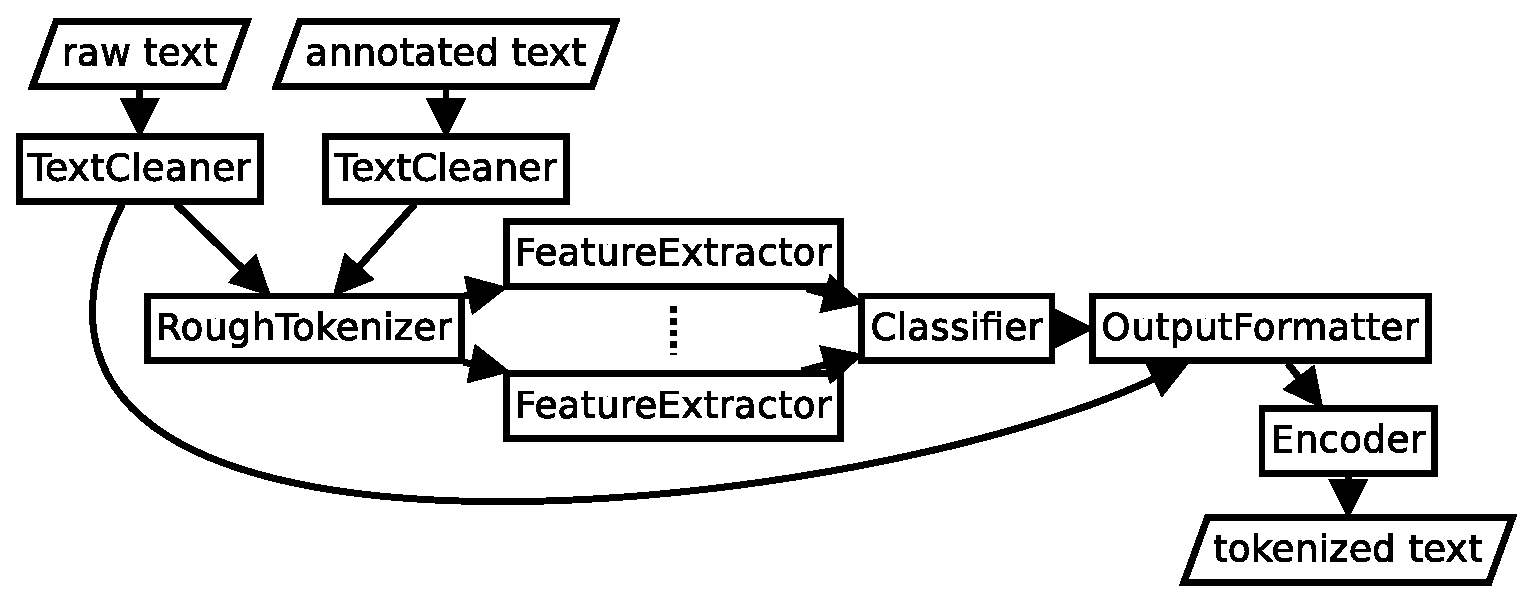
\includegraphics[width=\textwidth]{img/all-parts.eps}
  \caption{Data flow in the entire system}
  \label{fig:all-parts}
\end{figure}

\subsection{TextCleaner}

Any input which is read by the tokenizer is first processed with the
TextCleaner. This unit is responsible for decoding the stream of text and
optionally removing XML markup and expanding HTML entities and character
references. These changes to the input stream (referred to as cutouts in the
program) are conveyed to the OutputFormatter so that they can be undone in the
output. This allows the tokenizer to process XML marked up content as if it was
plaintext. The XML markup thus cannot be broken by and does not interfere with
the tokenization process.

\subsection{RoughTokenizer}

The RoughTokenizer's goal is to examine the cleaned input stream and identify
both unambiguous and ambiguous token and sentence boundaries. It does so by
splitting the text into what we call rough tokens. In the simplest case, rough
tokens are the whitespace delimited words of the text (the term word will be
used to mean a maximal subsequence of nonwhite characters). However, the user
can write regular expressions to define certain points within and between these
strings of nonwhite characters which may split them up into what end up being
the rough tokens. These user-defined points are called decision points and they
represent the ambiguous token/sentence boundaries.

There are three types of decision points. There is the \maysplit{} which occurs
within words and signals a potential token boundary. Then there is the
\maybreaksentence{} which occurs before and after certain characters and marks
a potential sentence boundary. \maysplit{} and \maybreaksentence{} are the
decision points which split words into rough tokens. The third type of decision
point is \mayjoin{} which occurs between words and turns the space between them
from a token boundary to a potential token boundary, making it possible for the
two words to join into a single token.

The rough tokenizer detects all decision points in the text can then be used
ane produces a stream of discrete rough tokens with metadata about surrounding
whitespace and decision points.

\subsection{FeatureExtractor}

The rough tokens produced by the RoughTokenizer are tagged with user-defined
properties in the FeatureExtractor. These predicate properties are defined
either using regular expressions or lists of rough tokens. In the case of a
regular expression, a rough token is said to have the property the expression
defines if and only if the regular expression matches the entire rough token.
When a property is defined using a token list, a rough token is said to have
the property if and only if it is on the list.

Because the task carried out by the FeatureExtractor is a context free function
of a single rough token's contents, multiple FeatureExtractors can run
simultaneously, each processing a different part of the token stream.

\subsection{Classifier}

The Classifier is the interface to the Maximum Entropy Toolkit. It scans the
rough token stream for decision points and collects evidential properties from
the tokens in the surrounding context. When the tokenizer is being trained, the
Classifier also reads in an annotated version of the input and aligns it with
the rough tokens (the annotated versions have one sentence per line with the
tokens delimited by spaces). It then bundles the values of the properties in
the context with the correct outcome inferred from the annotated data and sends
them both to the Maximum Entropy Toolkit for training. When a model is already
built and the tokenizer is tokenizing other data, it uses the context to query
the model for a predicted outcome and uses it to annotate the rough tokens. The
rough tokens are then processed by the OutputFormatter which implements the
token and sentece breaks predicted by the model.

\subsection{OutputFormatter}

After all the token and sentence boundaries have been disambiguated by the
Classifer, it is up to the OutputFormatter to convert the stream of rough
tokens into plain text where token boundaries are represented by spaces and
sentence boundaries by line breaks. It is also the duty of the OutputFormatter
to undo the changes done by the TextCleaner, which means that XML is reinserted
into the proper places and former HTML entities and character references
replace their expanded counterparts.

\subsection{Encoder}

The Encoder receives the text output by OutputFormatter and transcodes it from
the internal (UTF-8) encoding to the target encoding. In addition to changing
the coding of the characters, the Encoder and the TextCleaner also serve as
additional buffers for I/O operations so that the threads which run the
pipeline from RoughTokenizer to OutputFormatter are less likely to stall on
I/O.


\section{Modes of Execution}
\label{sec:impl-modes}

The tokenizer has to be trained on annotated data, it has to be able to use
that training to tokenize new input and it should also provide accurate
feedback on its performance when developing and evaluating a tokenization
scheme. The tokenizer thus has a few different setups for performing these
varied tasks.

\subsection{Training}

When the tokenizer is in the training mode, the only output it produces are
warning messages about token and sentence boundaries found in the annotated
version but not marked as potential boundaries in the raw input. This is a
signal to the user that he should perhaps modify the tokenization scheme to
account for more possible boundaries or to check his annotated data. The setup
of the system can be seen on figure~\ref{fig:train-parts}.

\begin{figure}
  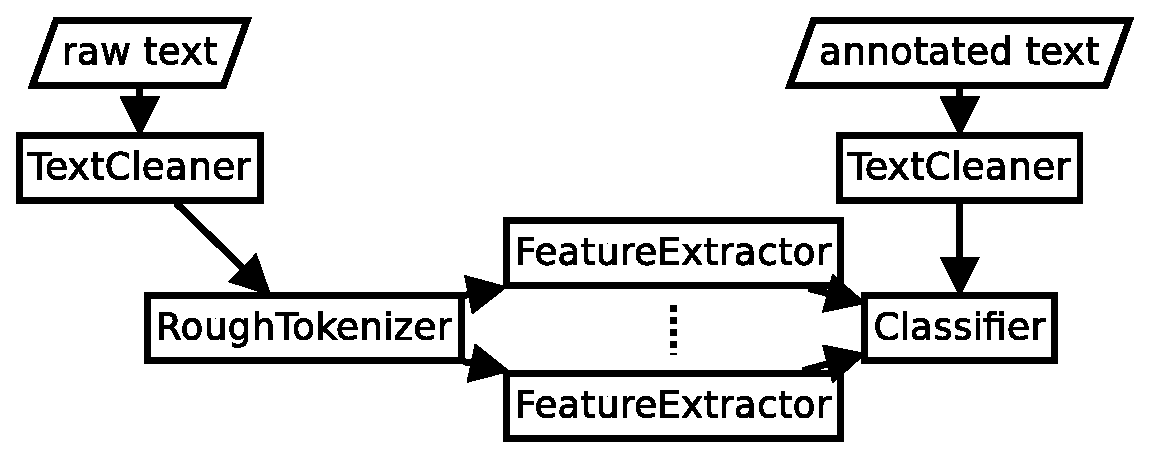
\includegraphics[width=\textwidth]{img/train-parts.eps}
  \caption{Data flow of the system in the training and evaluation
           configurations}
  \label{fig:train-parts}
\end{figure}

The Classifier is responsible for aligning the stream of rough tokens from the
input with the annotated text. The produced contextual information from the
tokens and the outcomes inferred from the aligned data are sent to the Maximum
Entropy Toolkit to serve as training data. After all the input files have been
processed and the training examples collected, the maximum entropy model is
computed and stored in a file for later use.

\subsection{Tokenization}

After a model has been trained, the tokenization mode becomes available. In
this mode the text is cleaned, converted into rough tokens and tagged with
properties. The Classifier has the trained model loaded and predicts the
outcome (sentence boundary, token boundary or no boundary) for every decision
point given its context. This outcome is used to resolve the \maysplit{},
\mayjoin{} and \maybreaksentence{} ambiguities and the disambiguation is stored
in the relevant rough token's metadata. These annotated tokens are then printed
through the OutputFormatter and encoded with the Encoder. See the setup of the
system in this mode on figure~\ref{fig:tokenize-parts}.

\begin{figure}
  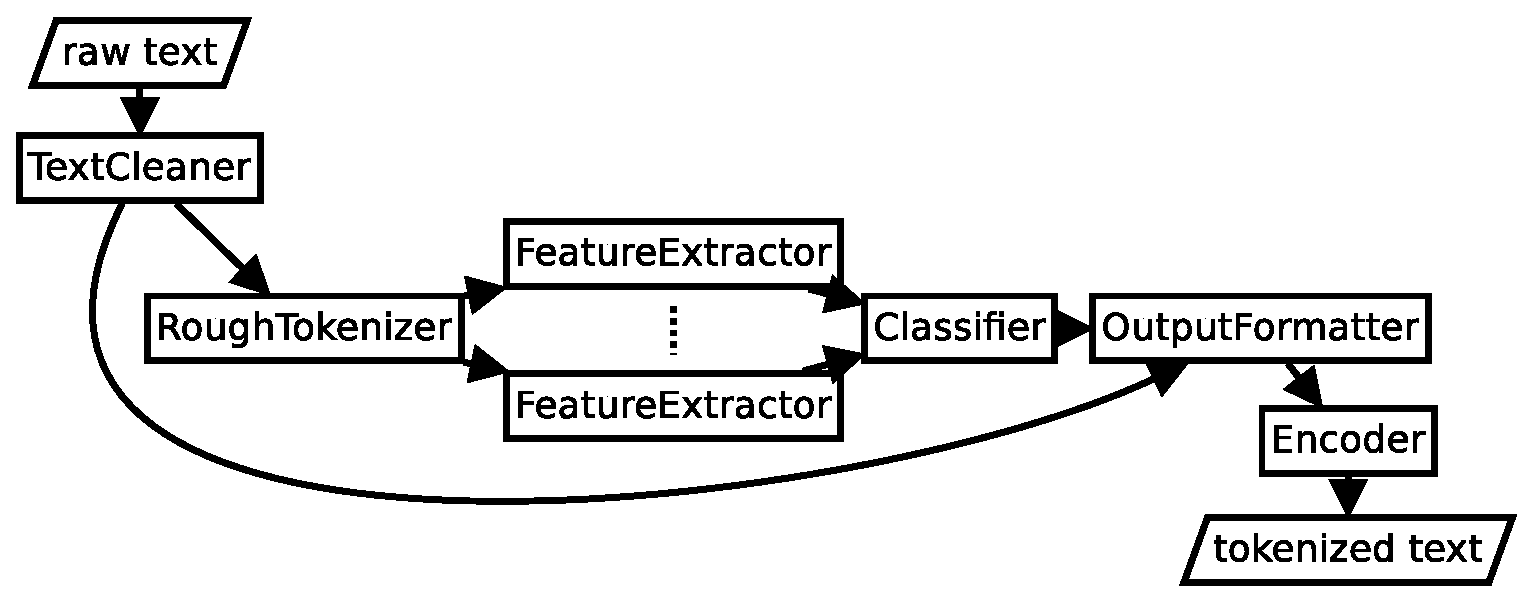
\includegraphics[width=\textwidth]{img/tokenize-parts.eps}
  \caption{Data flow of the system in the tokenization and preparation
           configurations}
  \label{fig:tokenize-parts}
\end{figure}

\subsection{Evaluation}

When tweaking and developing a tokenization system (the selected training data,
the configured parameters in the tokenization scheme) it is vital to have
feedback on the shortcomings of your system. The evaluation mode was designed
just for this purpose. It works in a way similar to the training mode (see
figure~\ref{fig:train-parts}). The Classifier aligns the rough tokens with the
annotated text and extracts the contextual properties from the tokens and the
true outcome from the annotated data. However, instead of recording them it
uses an already trained model and queries it for its predicted outcome. The
tokenizer then outputs both the true and the predicted outcome along with the
contextual properties.

Another tool can then be used to analyze the tokenizer's output and examine the
results and errors of the trained model. An example of such a tool would be the
included Python script analyze.py, which scans the evaluation's output and
reports the accuracy, precision, recall and F-measure of both sentence and
token boundary detection.

This log of outcomes and contexts can be written out when using any of the
available modes but only the evaluation mode has access to both the true
outcomes from the annotated data and the outcomes predicted by the
probabilistic model.

\subsection{Preparation}

The preparation is the last and least essential mode of the tokenizer. It is
similar to the tokenization mode (see figure~\ref{fig:tokenize-parts}), but
instead of querying the probabilistic model for an outcome, the Classifier
simply confirms all potential boundaries (\maysplit{} becomes a token boundary
and \maybreaksentence{} becomes a sentence boundary). This produces a file in
which an annotator only has to remove spaces and line breaks where
inappropriate to get the correct annotation.

An advantage to using this mode might be that when the user does not demand the
logging of contexts as in the evaluation mode, the time-costly FeatureExtractor
and Classifier can be replaced with a SimplePreparer, which only removes the
ambiguities in the abovementioned way.

\section{Rough Tokenization}
\label{sec:impl-roughtok}

One of the first problems encountered when designing the tokenizer was
the implementation of rough tokenization. The task of rough tokenization is to
take the definitions of decision points and then be able to detect all such
points in any given input.

The possible positions for a \maysplit{} decision point are defined by pairs
of regular expression: a poisition is to be marked as a \maysplit{} point if
and only if the first expression matches a suffix of the characters preceding
it and the second expression matches a prefix of the characters following it.
\mayjoin{} decision points are defined almost the same way, except that the
characters following the position of a \mayjoin{} must start with a string of
blank characters and then continue with the string matched by the regular
expression. \maybreaksentence{} points, on the other hand, are defined simply
by two sets of characters. If a position follows a character from the first
set or precedes a character from the second set, then that position is a
\maybreaksentence{}.

\subsection{Regular Expression Libraries}
\label{ssec:impl-roughtok-regex}

The reference implementation of the trainable tokenizer written in Perl used a
disjunction regular expression to match the prefix of the unprocessed input.
The original idea was to use PCRE or some other regular expression
implementation to write a similar algorithm.

The naive approach might have us trying to search for the possible suffixes of
\mayjoin{}s and \maysplit{}s which are preceded by their specified prefixes.
Soon we would learn that finding one decision point may lock us out of finding
another one. For example, given the string \example{abcd} and \maysplit{}
regular expression pairs \example{a} - \example{bc} and \example{b} -
\example{c}, we match the \example{bc} according to the leftmost longest match
convention properly registering the \maysplit{} between \example{a} and
\example{bc}, but we lose the opportunity to find the \maysplit{} between
\example{b} and \example{c}.

If try to search for each of these pairs of regular expressions individually,
we can still miss some points as demonstrated by the following example. Let the
string in question be \example{abab} and the \maysplit{} regular
expression pair \example{a} - \example{b(ab)*}. Any attempt to search for the
suffix \example{b(ab)*} would yield the \example{bab} substring due to the
leftmost longest match convention unless we either modify the user's regular
expression, modify the regular expression matching function or try to search
for the suffix from every position in the text.

We do not want to be patching the user's regular expressions because we would
probably have to restrict ourselves to a narrower set of regular expressions
and even then it would have been harrowing to actually implement such a system
and prove its correctness. Writing our own regular expression matching engine
is also out of the scope of this work. The third option on the list, searching
for the suffix (or prefix) from every position in the text, seems like a
performance killer. Performance-wise speaking, during the planning phase of
development, prototypes of the naive method of regular expression rough
tokenization were implemented using both Boost.Regex and PCRE. The average time
spent on a 10 MB file with a credible set of splitting and joining rules
(breaking English contractions apart, separating words from punctuation
etc...) was over 10.8 seconds for Boost.Regex and over 4.9 seconds using PCRE.
The test were performed on a development laptop with the Intel Core 2 Duo T7500
processor.

\subsection{Lexical Analyzer Generators}

During the initial planning, there was another radically different proposal for
handling rough tokenization which motivated the early prototypes.

The goal of rough tokenization is to scan large volumes of text and detect
patterns described by regular expressions. This kind of problem has been
already solved many times using lexical analyzer generators such as flex. These
tools take rules, which are pairs of regular expressions and actions written as
code. The lexical analyzer generator then creates a program from these rules
which reads a stream of text and tries to match a prefix of the yet unmatched
input with these regular expressions and reacts to the matches with the
supplied actions. More advanced tools enable the definition of several analyzer
modes with different rules and enables the actions to switch between them.

The lexical analyzer generator selected for our tokenizer was Quex. Its most
important feature is that it is able to work on Unicode code points instead of
single-byte characters and that it uses libiconv and ICU to process text in any
encoding. Quex can also be very fast because it does not encode the resulting
automaton into a table which drives some general template program, but instead
it generates low level C++ code which mimics the behaviour of the automaton.

The naive way of rough tokenization presented in
subsection~\ref{ssec:impl-roughtok-regex} was implemented in a prototype to
evaluate the performance benefits stemming from the use of compiled lexers
generated by Quex. When run with the same tokenization rules and on the same
data as the rough tokenizers in subsection~\ref{ssec:impl-roughtok-regex}, the
Quex generated lexer finished on average in a little over 0.9 seconds. But the
generated lexer was making the same mistakes as the first approaches using
regular expressions. As we grew to know more of the functionality available to
us in Quex and the specifics of its operation, we were able to arrive at a
lexer which detects every possible decision point and does so in about 1.9
seconds on the same data set with which we tested the other methods. The
details of this final method are presented in
subsection~\ref{ssec:impl-roughtok-solution}.

\subsection{The Solution}
\label{ssec:impl-roughtok-solution}

Many of the observations about the task at hand made in
subsection~\ref{ssec:impl-roughtok-regex} still hold when designing a Quex
generated lexer. The final implementation processes the input one character
at a time. At each position in the text, rules for matching the suffixes of
possible \maysplit{}s and \mayjoin{}s are in play. Each of these rules has a
precondition in Quex that the preceding text must match the prefix of the
respective \maysplit{} or \mayjoin{} rule. These aren't implemented by
backtracking and searching for the regular expression in the already processed
input. Instead, Quex maintains a set of flags which inform it which of the
preconditions are met at the current position. The \maybreaksentence{} rules
are implemented in a similar way as their definitions are basically
specializations of the \maysplit{} and \mayjoin{} definitions (single
characters for prefix or suffix instead of regular expressions).

When the lexer matches a suffix of a rule, it sends the last characters read
since the last decision point or whitespace as a rough token and signals the
respective decision point. Quex would now automatically adjust our position in
the text right behind the matched suffix but we override this behaviour and
move back to the position of the newly found decision point so other decision
points may be found. This alone would cause an infinite loop and so upon
returning to the original position we also scratch the detected decision point
from the set of applicable rules. If another decision point is found, we do the
same until we find all types of decision points at the current location or none
of the rules match anymore. In that case, the lowest priority action takes
place which reads another character from the stream and starts looking for all
possible decision points again.

This scratching out of rules is implemented using 8 different modes for all the
different sets of decision points we might be looking for. We start at the
topmost mode where we are looking for any of the 3 possible decision points. If
one of them is found, we continue at the same location in a mode which looks
for the remaining 2 possible decision points. In the final implementation,
there is also a demand for unexpanded HTML entities to be treated as single
rough tokens. This demand is met by adding another variable to the state of the
lexer (whether we are currently reading an entity) which results in the 16
modes seen in the current implementation.

\subsection{Technical Implementation}
\label{ssec:impl-roughtok-technical}

In the finished application, the regular expressions which define the placement
of decision points are read from user-written configuration files. A Quex
source file containing modes for detecting all of the decision points
referenced by the user is then output to a temporary file. CMake is invoked to
probe the user's system for the compiling essentials, to generate a project for
the user's preferred build system and to write the command needed to start the
build to a file. This file is read and the command within it is run, which
executes Quex on the generated source file and then compiles the result into a
shared module. This process is therefore platform-agnostic as it doesn't rely
on a specific C++ compiler or build system and uses only CMake and Quex which
are multiplatform and are required to build the tokenizer itself.

This compiled shared module is then loaded using the libtool's dynamic loading
library which is a wrapper for the platform-specific dynamic loading functions.
The entire code generation and compilation process takes under 5 seconds on the
development laptop. The tokenizer tracks the set of files used to generate the
rough tokenizer along with their timestamps and only regenerates and recompiles
it when changes have been made.

\section{Design Rationale}
\label{sec:impl-ratio}

\subsection{The Separation of Text Cleaning from Rough Tokenization}

When the first 
